% 1961 年全国卷第 9 题：由 A、B 方位与仰角测山高。
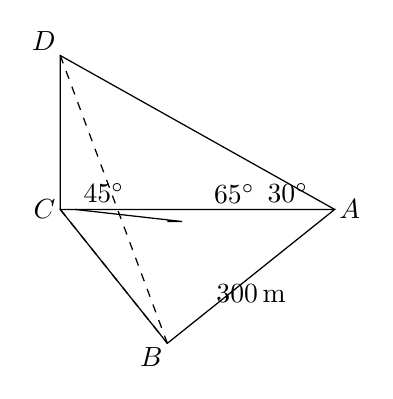
\begin{tikzpicture}[scale=0.85, line width=0.45pt,
  every node/.style={inner sep=1.5pt}]
  \coordinate (A) at (2.5,0.4);
  \coordinate (C) at (-1.6,0.4);
  \coordinate (D) at (-1.6,2.7);
  \coordinate (B) at (0.0,-1.6);
  \draw (A)--(B)--(C)--cycle;
  \draw (C)--(D)--(A);
  \draw[dashed] (C)--(B);
  \draw[dashed] (D)--(B);
  \draw (C)+(0.22,0)--(0.22,0.22)--(0,0.22);
  \node[anchor=west] at (A) {$A$};
  \node[anchor=north east] at (B) {$B$};
  \node[anchor=east] at (C) {$C$};
  \node[anchor=south east] at (D) {$D$};
  \node at (1.8,0.65) {$30^\circ$};
  \node at (1.0,0.63) {$65^\circ$};
  \node at (-0.95,0.65) {$45^\circ$};
  \node[anchor=north] at (1.25,-0.65) {$300\,\mathrm m$};
\end{tikzpicture}
